\documentclass[a4paper,12pt]{article}
\usepackage{xcolor}
\usepackage{amsmath,amsfonts,amssymb}
\usepackage{geometry}
\usepackage{fancyhdr}
\usepackage{graphicx}
\usepackage{titlesec}
\usepackage{tikz}
\usepackage{booktabs}
\usepackage{array}
\usetikzlibrary{shadows}
\usepackage{tcolorbox}
\usepackage{float}
\usepackage{lipsum}
\usepackage{mdframed}
\usepackage{pagecolor}
\usepackage{mathpazo}   % Palatino font (serif)
\usepackage{microtype}  % Better typography

\setlength{\parindent}{0pt}

% Page background color
\pagecolor{gray!10!white}

% Geometry settings
\geometry{margin=0.5in}
\pagestyle{fancy}
\fancyhf{}

% Fancy header and footer
\fancyhead[C]{\textbf{\color{blue!80}CS663 Assignment-4}}
% \fancyhead[R]{\color{blue!80}Saksham Rathi}
\fancyfoot[C]{\thepage}

% Custom Section Color and Format with Sans-serif font
\titleformat{\section}
{\sffamily\color{purple!90!black}\normalfont\Large\bfseries}
{\thesection}{1em}{}

% Custom subsection format
\titleformat{\subsection}
{\sffamily\color{cyan!80!black}\normalfont\large\bfseries}
{\thesubsection}{1em}{}

% Stylish Title with TikZ (Enhanced with gradient)
\newcommand{\cooltitle}[1]{%
  \begin{tikzpicture}
    \node[fill=blue!20,rounded corners=10pt,inner sep=12pt, drop shadow, top color=blue!50, bottom color=blue!30] (box)
    {\Huge \bfseries \color{black} #1};
  \end{tikzpicture}
}
\usepackage{float} % Add this package

\newenvironment{solution}[2][]{%
    \begin{mdframed}[linecolor=blue!70!black, linewidth=2pt, roundcorner=10pt, backgroundcolor=yellow!10!white, skipabove=12pt, skipbelow=12pt]%
        \textbf{\large #2}
        \par\noindent\rule{\textwidth}{0.4pt}
}{
    \end{mdframed}
}

% Document title
\title{\cooltitle{CS663 Assignment-4}}
\author{{\bf Saksham Rathi, Kavya Gupta, Shravan Srinivasa Raghavan} \\
\small Department of Computer Science, \\
Indian Institute of Technology Bombay \\}
\date{}

\begin{document}
\maketitle

\section*{Question 5}

\begin{solution}{Solution}
	Code is in \texttt{myMainScript.m}.

	We'll use $k = 75$ as it provided sufficiently good recognition rates in Q4.\ We see that the test error (minimum MSE) had mean around $77.7$ and standard deviation around $46.5$.

	\begin{center}
		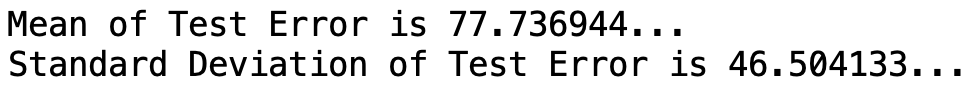
\includegraphics[scale=0.5]{../images/mean_std-dev.png}
	\end{center}

	So we propose that we look from $77.7 - 46.5 \approx 30$ to $77.7 + 4 \times 46.5 \approx 300$ for finding a suitable threshold.\ We took $4 \sigma$ to the right of mean so as to cover as many big test errors as possible.

	Basically we performed cross-validation to find the best threshold value.\ The metrics used to achieve this are:- Accuracy, F1-score, Youden's Index and one of my own.\ We maximise these metrics over the set of threshold values to find the best one.

	Note that here ``positives" are cases where a face is found to have a matching identity and ``negatives" are the opposite.\ $TP$ stands for ``True Positive'', $FP$ stands for ``False Positive'', $TN$ stands for ``True Negative'' and $FN$ stands for ``False Negative''.

	\begin{itemize}
		\item \textbf{Accuracy:}
		\[
			\text{Accuracy} = \frac{TP+TN}{TP+TN+FP+FN}
		\]
		Maximising Accuracy gives:-
		\begin{center}
			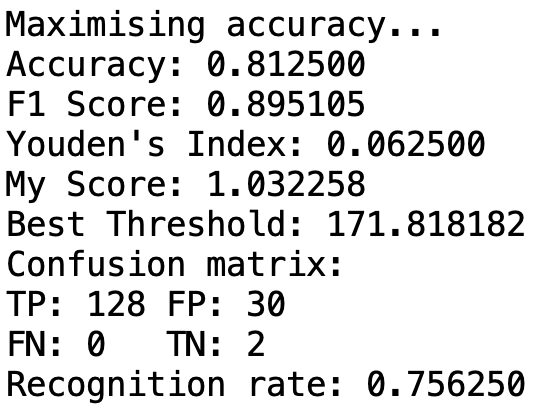
\includegraphics[scale=0.5]{../images/accuracy.png}
		\end{center}
		We see that the best threshold is around 172 and recognition rate is around 0.75 which is good.\ $FP$ is also not much.\ Hence this seems a good metric and a good threshold.
		\item \textbf{F1-score:}
		\[
			\text{F1-score} = \frac{2TP}{2TP+FP+FN}
		\]
		Maximising F1-score gives:-
		\begin{center}
			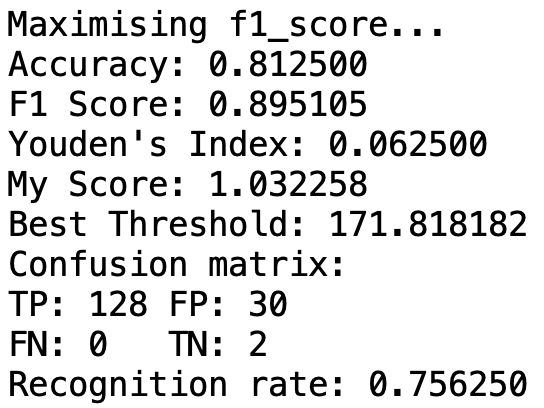
\includegraphics[scale=0.5]{../images/f1-score.png}
		\end{center}
		We see that the best threshold is around 172 and recognition rate is around 0.75 which is good.\ $FP$ is also not much.\ Hence this seems a good metric and a good threshold.
		\item \textbf{Youden's Index:}
		\[
			\text{Youden's Index} = \frac{TP}{TP+FN} + \frac{TN}{TN+FP} - 1
		\]
		Maximising Youden's Index gives:-
		\begin{center}
			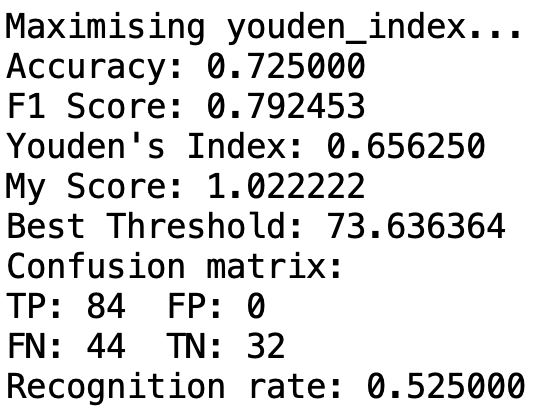
\includegraphics[scale=0.5]{../images/youden_index.png}
		\end{center}
		We see that the best threshold is around 73 and recognition rate is around 0.5 which is reasonable.\ Although $FP$ is 0, $FN$ is a little high.\ Though not very good, this is debatable.
		\item \textbf{My Metric:}
		\[
			\text{My Metric} = \frac{1}{FP+1} + \frac{1}{FN+1}
		\]
		Maximising my metric gives:-
		\begin{center}
			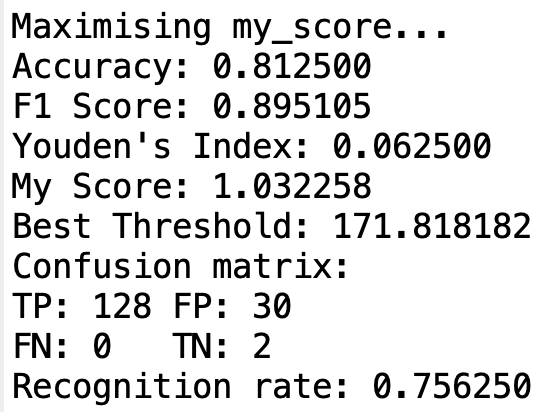
\includegraphics[scale=0.5]{../images/my-metric.png}
		\end{center}
		We see that the best threshold is around 172 and recognition rate is around 0.75 which is good.\ $FP$ is also not much.\ Hence this seems a good metric and a good threshold.
	\end{itemize}
	Hence, depending on the application we can choose any of the thresholds mentioned above. However, for general applications, where we would like to have a low number of False Positives and False Negatives, we can use a threshold value of 140 (as this is a value in between 73 and 172 and is closer to 172, hence best of both worlds).\ The results we get for a threshold of 140 are as follows:-
	\begin{center}
		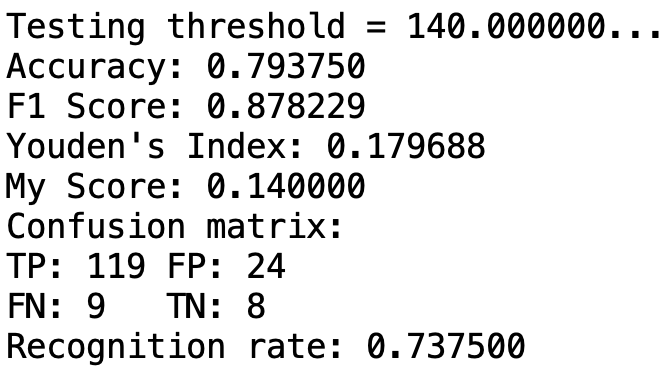
\includegraphics[scale=0.5]{../images/test.png}
	\end{center}
	Here we have 9 false negatives and 24 false positives.
\end{solution}




\end{document}
